\documentclass{standalone}
\usepackage{tikz}
\usetikzlibrary{shapes.geometric, positioning}
\tikzstyle{layer} = [rectangle, minimum width=8cm, draw=black, text centered]
\begin{document}
\begin{center}
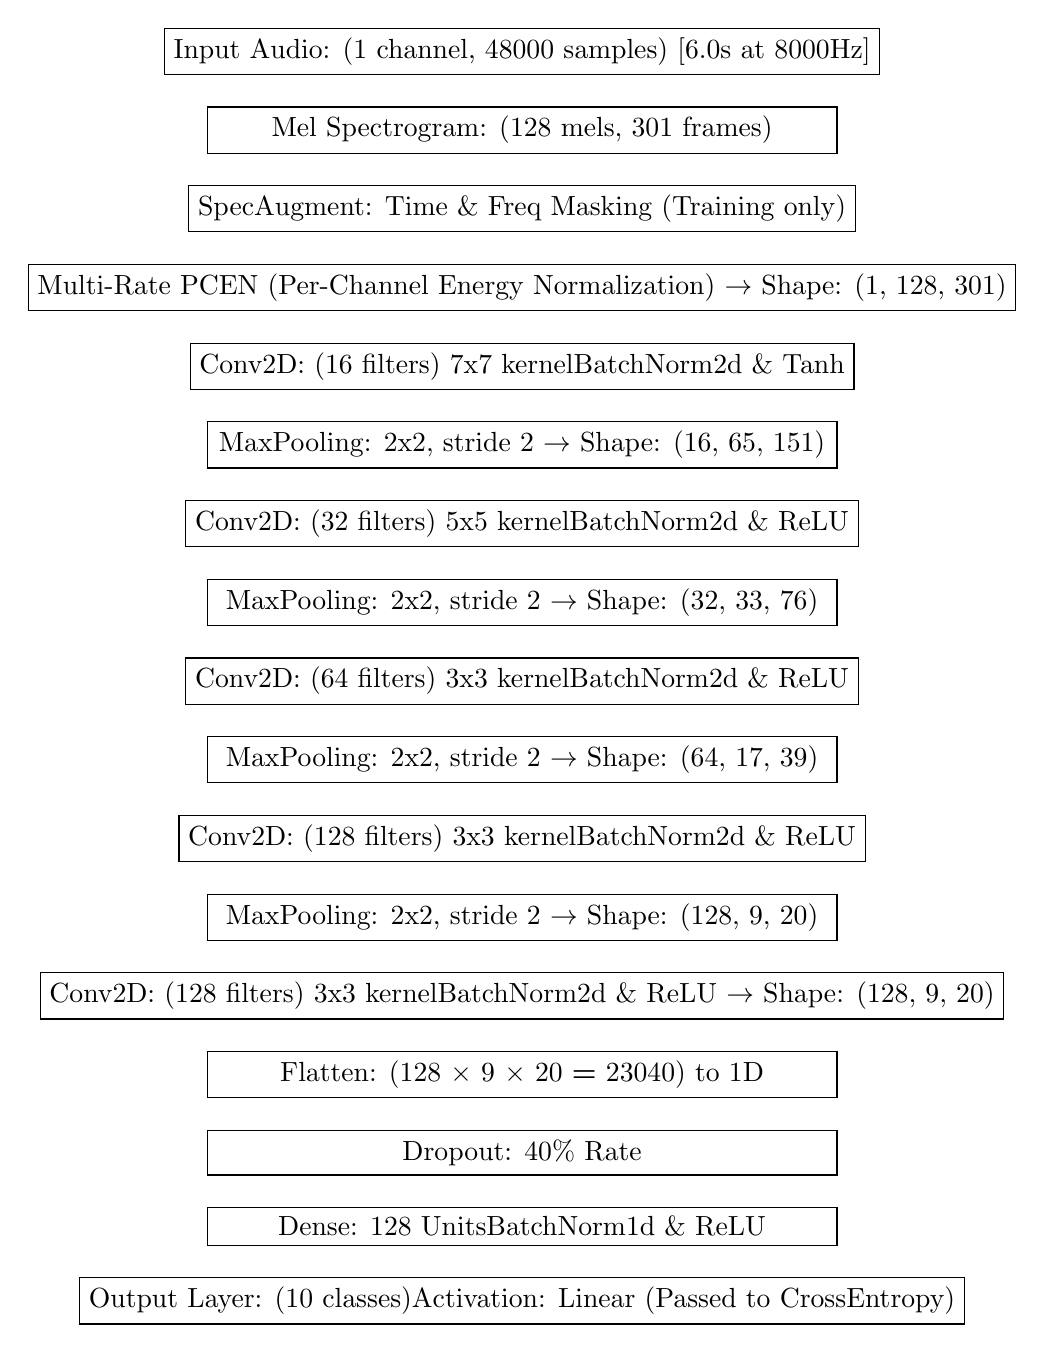
\begin{tikzpicture}[node distance=0.4cm] 

% Input Layer
\node[layer] (input) {Input Audio: (1 channel, 48000 samples) [6.0s at 8000Hz]};

% Mel Spectrogram
\node[layer, below=of input] (mel) {Mel Spectrogram: (128 mels, 301 frames)};

% SpecAugment + PCEN
\node[layer, below=of mel] (specaug) {SpecAugment: Time \& Freq Masking (Training only)};
\node[layer, below=of specaug] (pcen) {Multi-Rate PCEN (Per-Channel Energy Normalization) $\rightarrow$ Shape: (1, 128, 301)};

% First Convolution + MaxPooling
\node[layer, below=of pcen] (conv1) {Conv2D: (16 filters) 7x7 kernel \\ BatchNorm2d \& Tanh};
\node[layer, below=of conv1] (pool1) {MaxPooling: 2x2, stride 2 $\rightarrow$ Shape: (16, 65, 151)};

% Second Convolution + MaxPooling
\node[layer, below=of pool1] (conv2) {Conv2D: (32 filters) 5x5 kernel \\ BatchNorm2d \& ReLU};
\node[layer, below=of conv2] (pool2) {MaxPooling: 2x2, stride 2 $\rightarrow$ Shape: (32, 33, 76)};

% Third Convolution + MaxPooling
\node[layer, below=of pool2] (conv3) {Conv2D: (64 filters) 3x3 kernel \\ BatchNorm2d \& ReLU};
\node[layer, below=of conv3] (pool3) {MaxPooling: 2x2, stride 2 $\rightarrow$ Shape: (64, 17, 39)};

% Fourth Convolution + MaxPooling
\node[layer, below=of pool3] (conv4) {Conv2D: (128 filters) 3x3 kernel \\ BatchNorm2d \& ReLU};
\node[layer, below=of conv4] (pool4) {MaxPooling: 2x2, stride 2 $\rightarrow$ Shape: (128, 9, 20)};

% Fifth Convolution
\node[layer, below=of pool4] (conv5) {Conv2D: (128 filters) 3x3 kernel \\ BatchNorm2d \& ReLU $\rightarrow$ Shape: (128, 9, 20)};

% Flatten + Dropout + Dense
\node[layer, below=of conv5] (flatten) {Flatten: (128 $\times$ 9 $\times$ 20 \textbf{=} 23040) to 1D};
\node[layer, below=of flatten] (dropout) {Dropout: 40\% Rate};
\node[layer, below=of dropout] (dense) {Dense: 128 Units \\ BatchNorm1d \& ReLU};

% Output Layer
\node[layer, below=of dense] (output) {Output Layer: (10 classes) \\ Activation: Linear (Passed to CrossEntropy)};

\end{tikzpicture}
\end{center}
\end{document}
